\documentclass[twocolumn,10pt]{article}
\usepackage[pdftex]{graphicx}
%\usepackage{palatino}
\usepackage[osf]{mathpazo}
\usepackage{MnSymbol}
\usepackage{eprint}
%\usepackage{eco}
%\usepackage{amsfonts}
%\usepackage{amssymb}
\usepackage{latexsym}
\usepackage{microtype}
\usepackage{algorithmic}
\usepackage{ipe}

\DeclareMathAlphabet\mathbb{U}{msb}{m}{n}

\input{Qcircuit}

\newcommand{\braket}[2]{\langle #1|#2 \rangle}
\newcommand{\normtwo}{\frac{1}{\sqrt{2}}}
\newcommand{\norm}[1]{\parallel #1 \parallel}
\newcommand{\targfix}{\qw {\xy {<0em,0em> \ar @{ - } +<.39em,0em>
\ar @{ - } -<.39em,0em> \ar @{ - } +<0em,.39em> \ar @{ - }
-<0em,.39em>},<0em,0em>*{\rule{.01em}{.01em}}*+<.8em>\frm{o}
\endxy}}

%%%%%%%%%%%%%%%%%%%%%%%%%%%%%%%%%%%%%%%%%%%%%%%%%%%%%%%%%%%%%%%%%%%%%%%%%%%%%%
\title{Low-depth quantum architectures}

\author{Paul Pham}

\begin{document}

\maketitle

\begin{abstract}
In this report, we examine low-depth quantum architectures as a unifying
theme for classical control, parallelism in circuit construction,
error-correction, magic state distillation, and Hamiltonian simulation.
These topics have great importance both theoretically (in discovering
the limits of these techniques) and experimentally (in the efficient
implementation of algorithms). We examine uninitialized qubits
and approximate
algorithms and analyze the optimization of the QFT over time.
Since the low-depth trend has
bottomed out in many cases, resulting in a raft of
recent constant-depth circuits, we propose
future directions for quantum architecture research related to
circuit space, uncomputation, modular coherent states, and magic state
interconversion.
\end{abstract}

\section{Introduction}
\label{sec:intro}

Quantum computation has emerged as the most general model of what is
physically possible in our universe, redefining a computing machine as
making use of the full power of our most realistic theory of physics
at a small scale, quantum mechanics. However, great engineering challenges
currently stand between us and a fully working quantum computer, mostly
related to error correction, fault-tolerance, and maintaining delicate
control over microscopic systems while still interacting with them for
preparation and readout.

Some people have chosen to work on a more restrictive problem using
the quantum computing model of adiabatic optimization (cite D-Wave paper here).
The original and most popular model of universal quantum computing is the
quantum circuit model, which is what we examine in this report.
Quantum circuits, like their classical counterpart, consist of gates
whose inputs and outputs are connected to construct larger structures,
such that feeding in inputs in one end will give us our desired outputs at
the other end. In this case, however, the circuits are reversible.

Something about compiling also here, and references to
\cite{Pham2012a}. We define here quantum architecture as the physical
layout of qubits and their interactions in order to run quantum algorithms
while minimizing circuit resources \cite{VanMeter2006}, \cite{Pham2012b}.


In this report, we study an emerging trend in quantum circuit construction
research, that of low-depth quantum architectures, and we use it to unite
the important themes of classical control, parallelism, fault-tolerance,
and circuit resources. In doing so, we define several new resources to
augment the existing circuit model, namely \emph{circuit space}, its
combination with \emph{success probability}, and the use of
\emph{unitialized qubits}. Our approach is one of pragmatism with an
eye towards a new generation of quantum computer architects and engineers
working closely with both experimental physicsts and theorists to translate
algorithms onto running hardware.

Here then is the organization of our report.
In Section \ref{sec:circuit} we define the quantum circuit model and the
resources that are measured and minimized in quantum architecture. In
Section \ref{sec:qft} we apply this circuit model to the development of
a core building block, the quantum Fourier transform, and follow its
various optimizations over the years. In Section \ref{sec:factor} we
discuss the celebrated problem of factoring integers with a view to our new
model. In Section \ref{sec:parallel} we discuss some generic
parallelization techniques, due to Hoyer, Spalek, Takahashi, and Tani,
that have been behind the recent push towards constant-depth circuits.
In Section \ref{sec:ft} we discuss the connection of parallel classical
control and unitialized qubits to fault-tolerance and error-correcting codes.
In Section \ref{sec:magic} we find another unifying theme in the literature,
which is the source of a beautiful geometric perspective to UQC, called
magic state distillation. In Section \ref{sec:hamsim} we apply our model to
measure the performance of a useful problem in quantum computing,
namely that of simulating the Hamiltonian of a quantum system.
Finally, we conclude in Section \ref{sec:conclude} with some open problems
and interesting directions for future research to explore the themes developed
in this report.

%%%%%%%%%%%%%%%%%%%%%%%%%%%%%%%%%%%%%%%%%%%%%%%%%%%%%%%%%%%%%%%%%%%%%%%%%%%%%%
\subsection{The Rules of Quantum Mechanics}

An extensive background in quantum physics is not necessary to begin
working in and appreciating quantum computing or the work in this report.
The interested reader is referred to the standard textbook in this field
\cite{Nielsen2000}, but we will cover the mathematical basics here.
In general, quantum mechanics for the purposes of computing can be
explained in four rules.

Here I want to use Latex definitions with boldface for the terms, but I
forgot how to do that.

%%%%%%%%%%%%%%%%%%%%%%%%%%%%%%%%%%%%%%%%%%%%%%%%%%%%%%%%%%%%%%%%%%%%%%%%%%%%%%
\subsection{Rule 1: Qubits}

Rule 1 [Qubits]: Our basic unit of information is a quantum bit (\emph{qubit}),
a two-level system which can be represented by a column vector with
complex coefficients whose magnitudes squared sum to 1. These are known
as probability amplitudes for reasons which will become clear in Rule 4.
A quantum state
is written using Dirac bra-ket notation due to a visual pun for the
inner product, or the overlap between two quantum states.
The states $\ket{0}$ and $\ket{1}$ are known as the computational basis,
and correspond to our normal idea of classical bits.

\begin{equation}
\ket{\psi} = \alpha \ket{0} + \beta \ket{1} \qquad
|\alpha|^2 + |\beta|^2 = 1
\end{equation}

There is a nice correspondence between a single-qubit state and a geometric
picture known as the Bloch sphere, shown in Figure \ref{fig:bloch-sphere}.
We will return to this Bloch sphere picure later in talking about
magic state distillation in Section \ref{sec:magic}.
The north pole represents $\ket{0}$ and the south pole represents $\ket{1}$.

\begin{figure}
\label{fig:bloch-sphere}
\caption{The famous Bloch sphere}
\end{figure}

%%%%%%%%%%%%%%%%%%%%%%%%%%%%%%%%%%%%%%%%%%%%%%%%%%%%%%%%%%%%%%%%%%%%%%%%%%%%%%
\subsection{Rule 2: Tensor Product}

Individual qubits are not very useful, so we
can combine via the tensor product to form larger quantum
states. A two-qubit quantum state can exist as a complex superposition of
four two-bit classical states, still with probability amplitudes that sum to
one.

\begin{equation}
\ket{\psi} = \alpha \ket{00} + \beta \ket{01} + \gamma \ket{10} + \delta \ket{11}
\end{equation}

%%%%%%%%%%%%%%%%%%%%%%%%%%%%%%%%%%%%%%%%%%%%%%%%%%%%%%%%%%%%%%%%%%%%%%%%%%%%%%
\subsection{Rule 3: Unitary Operations}

Rule 3 [Unitary Operations]:
Qubits can be transformed by operations (also called \emph{gates})
that take the form of $2\times 2$ unitary matrices of unit determinant.
That is, they are reversible ($UU^\dagger = I$) and preserve the magnitude
of quantum states.

\begin{equation}
\left[ \begin{array}{cc}
a & b \\
c & d \\
\end{array} \right]
\end{equation}

%%%%%%%%%%%%%%%%%%%%%%%%%%%%%%%%%%%%%%%%%%%%%%%%%%%%%%%%%%%%%%%%%%%%%%%%%%%%%%
\subsection{Rule 4: Measurement}

Rule 3 [Measurement]: While a qubit can exist in a superposition
of computational basis states, when measured (that is, interacted with a
large macroscopic object like a human-sized scientific instrument), it
collapses to either $\ket{0}$ with probability $|\alpha|^2$ or
$\ket{1}$ with probability $|\beta|^2$.


\section{Quantum Circuit Resources}

Here we can mostly copy from my other papers, where I define quantum
architecture as being the connecting layer between quantum algorithms
and physical experiment. It's a really necessary connection, since otherwise
nice algorithms are ignored or unknown by experimentalists for lack of a
realistic mapping or being the resources are still too huge. Therefore, the
gains to be made in quantum architecture are usually not of the exponential
variety, but are polynomially gains asymptotically, which may turn out to be
huge in practice with actual constants. This may make the difference between
implementing a quantum computer in a few years versus several decades, if you
think we can sustain dramatic tension with DARPA / NSA / IARPA that long.

\subsection{The View}

I also mention here the field of quantum computer engineering, which will
include as its subfields quantum compilers (gate construction) and quantum
architecture (layout and error correction). I am mostly concerned

The tone of most of my paper is therefore more practically minded. Sometimes
mathematical formalism is necessary to realize substantial savings, but I will
not be overly concerned with nicely erasing my ancillae for the next algorithm
in line, especially if it means a large number of operations to uncompute it
to save a relatively small number of ancillae.

Also, I will stick to asymptotic improvements where possible, since these
statements are less likely to change over time or be dependent on
as-yet-unknown physical implementation. However, as an engineer I am still
impressed by numerical improvements, and on occasion I will use actual
constants to call out changes which would otherwise be lost in $O(\cdot)$
notation. This may be more appropriate in an intro section, which also
includes the rules of quantum computing.

\subsection{Circuit Resources}

In the traditional quantum circuit model, qubits are represented by lines,
and operations over the flow of time going from left to right. Of course,
due to the way matrix multiplication works, in real-life implementations,
the gates are applied going from right to left. Gates are represented by
blocks, and can be single-qubit (occurring on a single line) or
multi-qubit (spanning multiple lines).

\begin{figure}
\label{fig:circuit-resource.tex}
\caption{The circuit resources of width, depth, and size as described by others.}
\end{figure}

\emph{Circuit size} is the number of non-identity gates applied over time.
We specify non-trivial here, since in reality the identity gate may involve
extensive error-correction just to maintain a coherent quantum state over
a timestep, even without enacting any logical operation on it.
\emph{Circuit width} is the total number of qubits used in a computation,
including those storing the input and the output. It is fashionable in other
papers to only count ancillary qubits (ancillae), that is, the temporary 
scratch space used by the computation, which start out in the $\ket{0}$ state
and must be returned to it. This makes the circuit width smaller, and a more
impressive figure. However, this makes it hard to compare circuits
which compute the output in-place, ``on-top'' of the input qubits to save
space, to speak, versus those who compute out-of-place. Furthermore,
the output of one circuit is often the input to another, and in a practical sense,
we are interested in how many qubits we must physically maintain over time in
our experiment, and not whether these qubits store the inputs or outputs per se.
\emph{Circuit depth} is in some ways the most important figure. It describes
the number of parallel timesteps needed to complete a computation, given enough
parallel classical controllers. It provides a lower bound on the running time,
and like classical circuit depth, is analogous to the delay we can expect
from entering out inputs to getting a result.

Quantum architecture is primarily concerned with reducing circuit resources,
and previous approaches have concentrated on reducing circuit depth, circuit
width, or some combination of both (cite here the LNN factoring papers,
Van Meter's stuff).

\subsection{Architectural Models}

We follow here the terminology of Van Meter \cite{VanMeter2006} in his
definition of architectural models with different constraints, going from
very abstract but simple to more realistic but with more complicated constraints.

The qubits in the circuit models above are not
necessarily related spatially, and arbitrary interactions are allowed.
This is called the Abstract Concurrent (\textsc{AC}) model.

If we stipulate that the qubits then must be spatially related, in that
neighboring qubits in the circuit diagram are actually neighboring in real-life,
we take the natural shape of the entire arrangement of qubits to be in a line.
For the sake of realism, we only allow neighboring-qubits to interact, and we
only allow single-qubit and two-qubit gates. Due to various universality
proofs and fault-tolerance, it suffices to restrict ourselves to single-qubit
operations which are from the Clifford group and the $\pi/8$ gate and CNOT.
(Cite here Nielsen & Chuang, or KSV). We allow concurrent operations
acting on disjoint sets of qubits to occur within the same timestep.
This is called \textsc{1D-NTC}.

Next, it becomes natural to extend this model into two dimensions,

\section{Parallelization Techniques}
\label{sec:parallel}

Here we survey two powerful techniques behind a recent trend of work on
constant-depth circuits. The first is the constant-depth unbounded fan-out.
The second is the parallelization of
commuting gates and the so-called OR reduction of H{\o}yer and {\v S}palek
\cite{Hoyer2002}.

%%%%%%%%%%%%%%%%%%%%%%%%%%%%%%%%%%%%%%%%%%%%%%%%%%%%%%%%%%%%%%%%%%%%%%%%%%%%%%
\subsection{Unbounded Fanout}

In classical
circuits, the ability to copy bits is taken for granted. However,
in quantum circuits,
it is impossible to create an unentangled copy of a general quantum state, a
principle known as ``no-cloning'' \cite{Nielsen2000}. However,
it \emph{is} possible to create entangled copies by transversally applying
the CNOT gate to corresponding qubits in the source and destination register.
One can copy one source qubit $\ket{\psi} = \alpha \ket{0} + \beta \ket{1}$
to $n$ target qubits in this manner according to Equation \ref{eqn:copy}.

\begin{equation}
(\alpha \ket{0} + \beta \ket{1}) \otimes \ket{0}^{\otimes n} \rightarrow
\alpha \ket{0}^{\otimes (n+1)} + \beta \ket{1}^{\otimes (n+1)}
\end{equation}

This can be done in logarithic depth with a cascade of CNOTs as shown
in Figure \ref{fig:cnot-cascade}.

\begin{figure}
\label{fig:cnot-cascade}
\caption{A cascade of CNOTs implementing unbounded fan-out in logarithmic depth}
\end{figure}

Moore and Nilsson showed it was equivalent in power to the parity gate
\cite{Moore1998}. H{\o}yer and {\v S}palek have studied it in the
context of constant-depth circuits over a fixed basis ($\textsc{QNC}_f^0$)
to approximate AND, OR, MAJORITY, THRESHOLD$[t]$, and EXACT$[t]$ gates.

This has also been used in adder circuits by Takahashi and Tani
\cite{Takahashi2009} to achieve $O(\log^* n)$ depth.
These gates are not just of theoretical interest; some physical systems
such as ion traps admit the implementation of efficient multi-qubit gates,
following the work of M{\o}lmer and S{\o}rensen \cite{Sorensen1999}.
Recently unbounded fanout gates have also been implemented in 2D architectures using
constant-depth cat-state creation in $n$ ancillary qubits to
implement $n$-qubit controlled operations \cite{Rosenbaum2012} and
factoring in polylogarithmic-depth on a \textsc{2D NTC} architecture
\cite{Pham2012b}.
An $n$-qubit cat state is shown in Equation \ref{eqn:cat}; it is the
maximally entangled $n$-qubit state which is an equal superposition of all
$\ket{0}$'s and all $\ket{1}$'s.
However, unbounded fanout consumes the cat state,
in that it is not possible to uncompute the cat state after its use.

\begin{equation}
\label{eqn:cat}
\ket{\Phi_n} = \frac{1}{\sqrt{2}} \(\ket{0}^{\otimes n} + \ket{1}^{\otimes n}\)
\end{equation}

We describe how unbounded fanout can be used later to parallelize the
quantum Fourier transform in Section \ref{sec:qft}.

%%%%%%%%%%%%%%%%%%%%%%%%%%%%%%%%%%%%%%%%%%%%%%%%%%%%%%%%%%%%%%%%%%%%%%%%%%%%%%
\subsection{OR Reduction of Hoyer and Spalek}

Gate applied to different qubits can be applied at the same time. This is
the classical definition of parallelism

A key insight of Ref. \cite{Hoyer2002} is that any two commuting operations
can be performed as the same time, provided that (1) we have access to
unbounded fan-out and (2) that can efficiently transform
into the basis where they are both diagonal and that we have access.
This second condition is the case for many
functions needed in quantum algorithms, for example modular arithmetic
\cite{Moore1998}. This technique is exploited in their construction of
circuits for constant-depth rotation by Hamming weight and rotation by
Hamming value.

The essential concept between the OR reduction is to reduce computing the
OR of $n$ qubits to computing the OR of $\log n$ qubits in constant depth.
Once this has been done, one can apply the reduction recursively to reduce
the OR of $\log n$ qubits to the OR of $\log \log n$ qubits, until we
are left with a constant number of qubits that we can take the OR of
in the obvious way. In this manner, H{\o}yer and {\v S}palek get a circuit
of $O\log^* n}$ depth, where $\log^*n$ is the iterated logarithm function.

This technique was later extended by Takahashi and Tani to create an exact circuit
for OR in constant-depth. This resolves the open question of the power of
various constant-depth circuit complexity classes, namely.

\begin{equation}
\label{eqn:qcc}
\textsc{QNC}_f^0 = \textsc{QAC}_f^0 = \textsc{QTC}_f^0
\end{equation}

Equation \ref{eqn:qcc} is surprising because there is a separation between
the classical equivalents. Namely, 

\Ipe{pict/rotation-hamming.ipe}


\section{Quantum Fourier Transform}
\label{sec:qft}

We now apply the circuit resource model to a core building block of
many quantum algorithms: the quantum Fourier transform (QFT).

The QFT is responsible for most of our examples of an exponential quantum
speedup over classical algorithms. It was introduced in Shor's
original paper on finding prime factors and the discrete logarithm
\cite{Shor1995}, and it can be used to solve
other instances of the more general Hidden Subgroup Problem (HSP)
\cite{Lomont2004} over other finite Abelian groups \cite{Nielsen2000}.
It is now known
how to factor without the QFT,
using just phase estimation \cite{Kitaev2002} \cite{Cleve2000}, which may
be desirable due to the fine $\Lambda(R_k)$ controlled-phase rotations involved.
These are difficult to compile into an efficient, fault-tolerant, universal
gateset since it involves non-Clifford single-qubit rotations $\Lambda(e^{i\theta})$.

\begin{equation}
\label{eqn:rk}
\Lambda(R_k) = \left[ \begin{array}{cccc}
1 & 0 & 0 & 0\\
0 & 1 & 0 & 0\\
0 & 0 & 1 & 0\\
0 & 0 & 0 & e^{i\pi / 2^k}
\end{array}
\right]
\end{equation}

However, the QFT is still of practical importance
in determining the
properties of quantum chemical systems
(such as their ground state energies) \cite{Wang2008} as well as in
many algorithms of the late 90s such as
the transform adder by Draper \cite{Draper2000} and extensions to Grover's
search algorithm \cite{Grover1996} \cite{Brassard1998} \cite{Mosca1999}.
While this gives the QFT somewhat of a vintage feel within the community,
it is still a venerable, useful technique.
Therefore, it makes an ideal candidate for analyzing its depth optimization
over the years, using the techniques
of approximation and unbounded fan-out.

In the rest of this section,
we will show how the QFT has been parallelized and its depth decreased from the
initial quadratic
value \ref{subsec:qft-quad} down to
log-linear \ref{subsec:qft-loglin},
linear \ref{subsec:qft-linear}, and logarithmic depth \ref{subsec:qft-log},
as well as circuit space and its error probability, where
appropriate. 

%%%%%%%%%%%%%%%%%%%%%%%%%%%%%%%%%%%%%%%%%%%%%%%%%%%%%%%%%%%%%%%%%%%%%%%%%%%%%%
\subsection{The Discrete Fourier Transform}

As the name implies, the QFT is inspired by the classical, discrete
Fourier transform (DFT) which relates two sets of complex numbers
$\{x_0, x_1, \ldots, x_{N-1}\}$ and $\{y_0, y_1, \ldots, y_{N-1}\}$,
each in different domains.

\begin{equation}
y_k \equiv \frac{1}{\sqrt{N}} \sum_{j=0}^{N-1} x_j e^{2\pi i j k / N}
\label{eqn:dft}
\end{equation}

This is the idea behind the fast Fourier transform (FFT) \cite{Cooley1965}
used in fast
integer multiplication, fast matrix multiplication \cite{Schoenhage1971},
and many other
important applications \cite{Maslen1997}. The QFT performs a different
operation on quantum states, namely it converts between two bases of
quantum states,
say $\{\ket{j}\}$ and $\{\ket{k}\}$, where usually one of these bases is
the computational basis $\{\ket{0}, \ket{1}, \ldots, \ket{N-1}\}$
and the other we call the \emph{Fourier basis}. The complex amplitudes
$x_j$ of a
particular $\ket{j}$ are related to the amplitudes $y_k$ of all the $\ket{k}$
by the discrete Fourier transform in Equation \ref{eqn:dft}.

\begin{equation}
\ket{j} = \frac{1}{\sqrt{N}} \sum_{k=0}^{N-1} e^{2\pi i j k / N} \ket{k}
\end{equation}

\begin{equation}
\sum_{j=0}^{N-1} x_j \ket{j} \rightarrow \sum_{k=0}^{N-1} y_k \ket{k}
\end{equation}

The relationship between the QFT and the DFT can be thought of as the
difference between computing all the probabilities of a certain distribution
and just sampling from a distribution \cite{Cleve2000}. The latter problem is
often much easier. In both cases, we speak of computing the Fourier transform
with respect to the modulus $N$, the number of basis elements.

The application of the QFT in most quantum algorithms
involve encoding some useful information about each state into its phase,
so that after applying the QFT or its inverse, the correct answer is measured
with high probability.

%%%%%%%%%%
% FIGURE %
%%%%%%%%%%
%\begin{figure}
%\caption{Sound recording in the time and frequency domains}
%\end{figure}

%By analogy, in many quantum algorithms we can encode useful information
%into the phases associated with the probability amplitudes of different
%computational basis states. Our usual goal is to interfere these phases
%both constructively and destructively, to maximize the probability of measuring
%the computational basis state that corresponds to a correct answer to our
%problem. The restriction is that we can only do this using local operations,
%that, by operating on a few neighboring qubits at a time. Through this means,
%we are effectively operating on many computational basis states in parallel,
%due to the way quantum states combine through the tensor product structure.

%[somewhere in the previous section, i unveil my famous spectrum picture
%of quantum states, and demonstrate some examples of highly-entangled
%states and product states]

%%%%%%%%%%%%%%%%%%%%%%%%%%%%%%%%%%%%%%%%%%%%%%%%%%%%%%%%%%%%%%%%%%%%%%%%%%%%%%
\subsection{The Product Representation}

%In one domain, we have information encoded in the bits of the computational
%basis states, but these are just encodings, and you can imagine them
%evolving happily in their own separate alternate universes until one of them
%is selected by random chance by a measurement at the end.
%In the second domain, we have the phases of each computational basis state,
%and the way we can get different computational basis states to interact, or
%to create more or less of them, is through two-qubit entangling gates.
%Actually, now we are on thin ice, and I should think carefully about what I
%want to say here, especially as it relates to universality.

Due to the tensor product structure of multi-qubit quantum states, we can
perform the QFT by performing single-qubit and controlled-phase two-qubit
rotations (the $R_k$ from Equation \ref{eqn:rk}). To do this, imagine that
we have an $n$-qubit computational basis state $\ket{j}$ where
qubit $\ket{j_i}$ has significance $2^i$ in our encoding. We now define the
following single-qubit state with a rotation based on the binary fraction
using bits $j_\ell$ through $j_n$, where $0.j_{\ell} j_{\ell-1} \ldots j_{n} =
\sum_{m=\ell}^n 2^{-m}j_m$.

\begin{equation}
\ket{\phi(\ell)} = \frac{1}{\sqrt{2}}\left( \ket{0} +
e^{2\pi i 0.j_\ell j_{\ell-1} \ldots j_n} \ket{1} \right)
\end{equation}

We can enact each $\ket{\phi(\ell)}$ by using $n-\ell$ rotations
$R_k$ from Equation \ref{eqn:rk} controlled on qubits $\ket{j_\ell}$
through $\ket{j_n}$.

We can then express the QFT on a computational basis state $\ket{j}$ as
the following tensor product of rotated single-qubit states, as proved in
\cite{Nielsen2000}.

\begin{equation}
\ket{j_1, j_2, \ldots, j_n} = \bigotimes_{\ell=1}^{n} \ket{\phi(\ell)}
\end{equation}

%\begin{figure}
%\caption{My famous rotating phase wheel picture}
%end{figure}

We note here that all the QFT circuits we will be discussing in this section
assume the modulus is a power of two, namely $N=2^n$. In reality, we may
approximate arbitrary moduli $m$ with $n'$ qubits where
$n' = \lfloor\log m\rfloor + O(1)$ to within error $\epsilon$, which determines
the circuit size and depth polynomially in $1/\epsilon$
as described in \cite{Cleve2000}.

%%%%%%%%%%%%%%%%%%%%%%%%%%%%%%%%%%%%%%%%%%%%%%%%%%%%%%%%%%%%%%%%%%%%%%%%%%%%%%
\subsection{QFT in $O(n^2)$ Depth}
\label{subsec:qft-quad}

The most well-known circuit for the QFT from Nielsen \& Chuang
\cite{Nielsen2000} applies each of the following gates in sequence, as shown
in Figure \ref{fig:qft-serial}.

For each qubit in $\ket{j_\ell}$, apply a Hadamard gate to get an equal mix of
$\ket{0}$ and $\ket{1}$ for subsequence rotations. Then apply $n-\ell-1$
$R_k$ rotations targeting $\ket{j_\ell}$ controlled on bits $\ket{j_{\ell+1}}$
to $\ket{j_n}$, where qubit $\ket{j_m}$ controls a rotation $R_{m-\ell+1}$.

\begin{figure}[h!]
\begin{center}
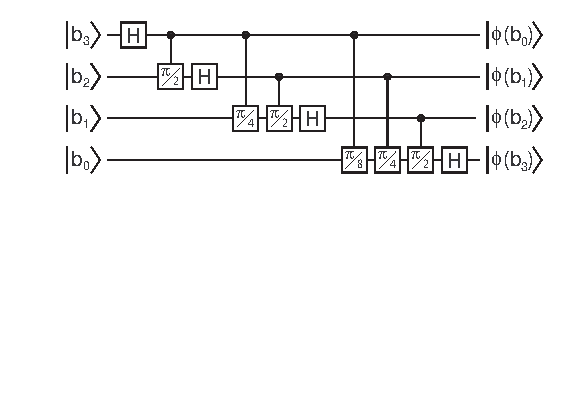
\includegraphics[width=3in]{figures/serial_qft.pdf}
\caption{The serial QFT circuit \cite{Fowler2004}.}
\label{fig:qft-serial}
\end{center}
\end{figure}

%\begin{equation}
%\label{eqn:qft-quad}
%\end{equation}

The depth and size of operations are calculated as
$\sum_{\ell=1}^n n-\ell-1 = O(n^2)$.
Also note that no ancillary qubits are needed, and the QFT is computed
in-place. Therefore the circuit width is $n$, and the circuit space is
$O(n^3)$ with an error probability of $0$ since this is an exact circuit.

%%%%%%%%%%%%%%%%%%%%%%%%%%%%%%%%%%%%%%%%%%%%%%%%%%%%%%%%%%%%%%%%%%%%%%%%%%%%%%
\subsection{QFT in $O(n\log n)$ Depth}
\label{subsec:qft-loglin}

Almost immediately after Shor's original paper, Coppersmith noted that we
could cut off the rotations $R_k$ after some maximum $k_0 = O(\log(n/\epsilon))$
and therefore decrease
our circuit size and depth to $O(n\log(n/\epsilon))$ for a given
error $\epsilon$ \cite{Coppersmith1994}. We will call this the AQFT,
for \emph{approximate QFT}. For circuits of size polynomial
in $n$, it suffices to set $\epsilon = 1/poly(n)$, and therefore our
circuit size and depth is $O(n\log(n))$. The circuit width remains the same
as before, so the circuit space is now $O(n^2\log(n))$ for
error probability $1/poly(n)$.

%%%%%%%%%%
% FIGURE %
%%%%%%%%%%
%\begin{figure}
%\label{fig:qft-approx}
%\caption{Circuit for the approximate QFT}
%\end{figure}

%%%%%%%%%%%%%%%%%%%%%%%%%%%%%%%%%%%%%%%%%%%%%%%%%%%%%%%%%%%%%%%%%%%%%%%%%%%%%%
\subsection{QFT in $O(n)$ Depth}
\label{subsec:qft-linear}

It was noted by Moore and Nilsson \cite{Moore1998} and widely attributed
to folklore that the QFT would be further parallelized by swapping qubits
so that $R_k$ rotations that operated on disjoint qubits could be executed
in the same timestep. Incidentally, this also makes the QFT implementable
on a nearest-neighbor architecture, which was discovered by Kutin, Devitt,
and Hollenberg \cite{Fowler2004} to have a pleasing triangular shape
as shown in Figure \ref{fig:qft-parallel}. This fact was later
used in the 1D NTC
architecture of Kutin \cite{Kutin2006}.

%%%%%%%%%%
% FIGURE %
%%%%%%%%%%
\begin{figure}
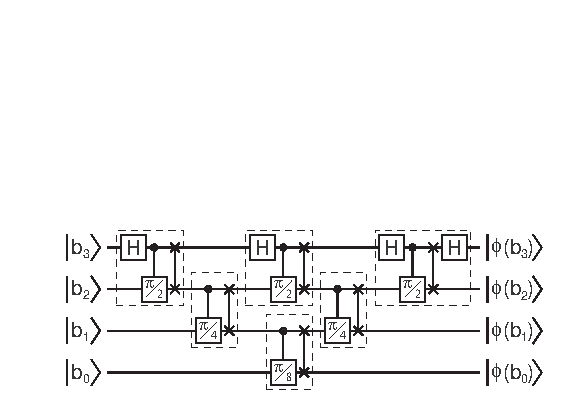
\includegraphics[width=3in]{figures/parallel_qft.pdf}
\caption{The parallel 1D NTC QFT circuit \cite{Fowler2004}.}
\label{fig:qft-parallel}
\end{figure}

This reduces the depth to $O(n)$, while the size and width remain the same
as before. Therefore, the circuit space is now $O(n^2)$, an improvement over
the AQFT in the previous section but with an error probability of $0$ since
this is an exact circuit.

%%%%%%%%%%%%%%%%%%%%%%%%%%%%%%%%%%%%%%%%%%%%%%%%%%%%%%%%%%%%%%%%%%%%%%%%%%%%%%
\subsection{QFT in Depth $O(\log n)$}
\label{subsec:qft-log}

To further exploit the fact that operations on disjoint qubits can be done
in parallel, Cleve and Watrous discovered that one could fanout the control
qubit of every $R_k$ rotation. This uses the copying technique of
Section \ref{sec:parallel}, which uses a logarithmic-depth \emph{copy network}
of
CNOT gates to create $\ell-1$ entangled copies of a source qubit
$\ket{j_\ell}$. Now every rotation controlled on $\ket{j_\ell}$ can be done
in parallel, as shown in Figure \ref{fig:qft-cw}. We can combine
this to use the
result of the approximate QFT to cut off rotations after $\log(n/\epsilon)$
bits.

\begin{figure}[!ht]
\rule{1cm}{0cm}
\setlength{\unitlength}{965sp}%
%
\begingroup\makeatletter\ifx\SetFigFont\undefined
% extract first six characters in \fmtname
\def\x#1#2#3#4#5#6#7\relax{\def\x{#1#2#3#4#5#6}}%
\expandafter\x\fmtname xxxxxx\relax \def\y{splain}%
\ifx\x\y   % LaTeX or SliTeX?
\gdef\SetFigFont#1#2#3{%
  \ifnum #1<17\tiny\else \ifnum #1<20\small\else
  \ifnum #1<24\normalsize\else \ifnum #1<29\large\else
  \ifnum #1<34\Large\else \ifnum #1<41\LARGE\else
     \huge\fi\fi\fi\fi\fi\fi
  \csname #3\endcsname}%
\else
\gdef\SetFigFont#1#2#3{\begingroup
  \count@#1\relax \ifnum 25<\count@\count@25\fi
  \def\x{\endgroup\@setsize\SetFigFont{#2pt}}%
  \expandafter\x
    \csname \romannumeral\the\count@ pt\expandafter\endcsname
    \csname @\romannumeral\the\count@ pt\endcsname
  \csname #3\endcsname}%
\fi
\fi\endgroup
\begin{picture}(8910,5495)(376,-6744)
\thinlines
\put(4801,-3061){\circle*{150}}
\put(4801,-3661){\circle*{150}}
\put(4801,-1561){\circle*{150}}
\put(4801,-2461){\circle*{150}}
\put(4801,-2161){\circle{150}}
\put(4801,-2761){\circle{150}}
\put(4801,-3361){\circle{150}}
\put(4801,-3961){\circle{150}}
\put(4801,-1561){\line( 0,-1){675}}
\put(4801,-2461){\line( 0,-1){375}}
\put(4801,-3061){\line( 0,-1){375}}
\put(4801,-3661){\line( 0,-1){375}}
\put(4201,-1561){\circle*{150}}
\put(4201,-3061){\circle*{150}}
\put(4201,-3661){\circle{150}}
\put(4201,-2461){\circle{150}}
\put(4201,-1561){\line( 0,-1){975}}
\put(4201,-3061){\line( 0,-1){675}}
\put(3601,-1561){\circle*{150}}
\put(3601,-3061){\circle{150}}
\put(3601,-1561){\line( 0,-1){1575}}
\put(7201,-3061){\circle*{150}}
\put(7201,-3661){\circle*{150}}
\put(7201,-1561){\circle*{150}}
\put(7201,-2461){\circle*{150}}
\put(7201,-2161){\circle{150}}
\put(7201,-2761){\circle{150}}
\put(7201,-3361){\circle{150}}
\put(7201,-3961){\circle{150}}
\put(7201,-1561){\line( 0,-1){675}}
\put(7201,-2461){\line( 0,-1){375}}
\put(7201,-3061){\line( 0,-1){375}}
\put(7201,-3661){\line( 0,-1){375}}
\put(7801,-1561){\circle*{150}}
\put(7801,-3061){\circle*{150}}
\put(7801,-3661){\circle{150}}
\put(7801,-2461){\circle{150}}
\put(7801,-1561){\line( 0,-1){975}}
\put(7801,-3061){\line( 0,-1){675}}
\put(8401,-1561){\circle*{150}}
\put(8401,-3061){\circle{150}}
\put(8401,-1561){\line( 0,-1){1575}}
\put(5401,-4561){\circle*{150}}
\put(5551,-4861){\circle*{150}}
\put(5701,-5161){\circle*{150}}
\put(5851,-5461){\circle*{150}}
\put(6001,-5761){\circle*{150}}
\put(6151,-6061){\circle*{150}}
\put(6301,-6361){\circle*{150}}
\put(6451,-6661){\circle*{150}}
\put(5401,-1561){\circle*{150}}
\put(5551,-2161){\circle*{150}}
\put(5701,-2461){\circle*{150}}
\put(5851,-2761){\circle*{150}}
\put(6001,-3061){\circle*{150}}
\put(6151,-3361){\circle*{150}}
\put(6301,-3661){\circle*{150}}
\put(6451,-3961){\circle*{150}}
\put(2401,-1861){\framebox(600,600){\large H}}
\put(1801,-1561){\line( 1, 0){600}}
\put(5401,-1561){\line( 0,-1){3000}}
\put(5551,-2161){\line( 0,-1){2700}}
\put(5701,-2461){\line( 0,-1){2700}}
\put(5851,-2761){\line( 0,-1){2700}}
\put(6001,-3061){\line( 0,-1){2700}}
\put(6151,-3361){\line( 0,-1){2700}}
\put(6301,-3661){\line( 0,-1){2700}}
\put(6451,-3961){\line( 0,-1){2700}}
\put(3001,-1561){\line( 1, 0){6000}}
\put(1801,-2161){\line( 1, 0){7200}}
\put(1801,-2461){\line( 1, 0){7200}}
\put(1801,-2761){\line( 1, 0){7200}}
\put(1801,-3061){\line( 1, 0){7200}}
\put(1801,-3361){\line( 1, 0){7200}}
\put(1801,-3661){\line( 1, 0){7200}}
\put(1801,-3961){\line( 1, 0){7200}}
\put(1801,-4561){\line( 1, 0){7200}}
\put(1801,-4861){\line( 1, 0){7200}}
\put(1801,-5161){\line( 1, 0){7200}}
\put(1801,-5461){\line( 1, 0){7200}}
\put(1801,-5761){\line( 1, 0){7200}}
\put(1801,-6061){\line( 1, 0){7200}}
\put(1801,-6361){\line( 1, 0){7200}}
\put(1801,-6661){\line( 1, 0){7200}}
\put(9500,-1681){\makebox(0,0)[lb]{$\ket{\mu_{0.x_j\cdots x_0}}$}}
\put(9500,-3166){\makebox(0,0)[lb]{$\ket{0^{j}}$}}
\put(9500,-4700){\makebox(0,0)[lb]{$\ket{x_j}$}}
\put(800,-4700){\makebox(0,0)[lb]{$\ket{x_j}$}}
\put(9600,-5700){\makebox(0,0)[lb]{$\vdots$}}
\put(900,-5700){\makebox(0,0)[lb]{$\vdots$}}
\put(800,-6800){\makebox(0,0)[lb]{$\ket{x_0}$}}
\put(9500,-6800){\makebox(0,0)[lb]{$\ket{x_0}$}}
\put(800,-3166){\makebox(0,0)[lb]{$\ket{0^{j}}$}}
\put(800,-1681){\makebox(0,0)[lb]{$\ket{0}$}}
\end{picture}\vspace{2mm}
\caption{QFT circuit in $O(\log n)$ depth due to Cleve and Watrous \cite{Cleve2000}.}
\label{fig:qft-cw}
\end{figure}

Furthermore, each copy network for all $n$ bits $\ket{j_\ell}$ can be done
in parallel.
Therefore, the circuit's depth is now only limited by the copy networks
and is now $O(\log n)$. The size remains unchanged asymptotically, but now
the circuit width is $O(n^2)$ to include the ancillae for the copy networks.
The circuit space is therefore $O(n^3\log\log(n/\epsilon)$. The size and
error probability is
the same as the AQFT.

%%%%%%%%%%%%%%%%%%%%%%%%%%%%%%%%%%%%%%%%%%%%%%%%%%%%%%%%%%%%%%%%%%%%%%%%%%%%%%
\subsection{QFT Summary}

Table \ref{tab:qft-summary} summarizes the circuit size, depth, width, space, and
error probability for the QFT implementations discussed in this section.
For the approximate circuits, we set $\epsilon = 1/O(n^2)$,
since this is the per-gate error we would need to get a constant
error probability for a QFT on $n$ qubits.

\begin{figure*}
\begin{center}
\begin{tabular}{|c|c|c|c|c|c|}
\hline
\textbf{Author} & \textbf{Depth} & \textbf{Size} & \textbf{Width} & \textbf{Space} & \textbf{Error}\\
\hline
Shor & $O(n^2)$ & $O(n^2)$ & $O(n)$ & $O(n^3)$ & 0\\
Coppersmith & $O(n\log n)$ & $O(n\log n)$ & $O(n)$ & $O(n^2\log n)$ & $1/O(n^2)$ \\
Folklore & $O(n)$ & $O(n^2)$ & $O(n)$ & $O(n^2)$ & 0\\
Cleve-Watrous & $O(\log n)$ & $O(n^2)$ & $O(n^2)$ & $O(n^2 \log n)$ & 0\\
Cleve-Watrous & $O(\log \log n)$ & $O(n \log n)$ & $O(n^2)$ & $O(n^2 \log\log n)$ & $1/O(n^2)$\\
Browne-Kasheffi-Perdrix & $O(1)$ & $O(n^2)$ & $O(n^2)$ & $O(n^2)$ & 0\\
\hline
\end{tabular}
\caption{Summary of circuit resources for different QFT implementations.}
\label{tab:qft-summary}
\end{center}
\end{figure*}

The result of Browne et al. \cite{Browne2009} replaces the copy network
of Cleve and Watrous with a constant-depth unbounded fan-out.
BKP can also be used to implement an
AQFT with improved circuit space, but there is no further depth improvement
possible. By introducing circuit space, we hope to provide another parameter
for continuing to improve QFT circuits in the future that will affect
practical implementations.


\section{Factoring}
\label{sec:factor}

Shor's factoring algorithm in 1994 was the first and most famous example of an
exponential speedup of quantum computers over classical computers.
\cite{Shor1994}
As such, it is still an active area of research, both in optimizing the
circuit \cite{Cleve2002} and the experimental implementation. (actually,
I don't know of any
recent experiments that are getting close to doing this again).

Although we study this problem in greater depth in a separate work
\cite{Pham2012b}, we mention here some interesting techniques introduced
specifically for factoring but which may have wider applications.

\subsection{Modular Entangled States}

In most quantum computations, qubits become part of a larger and larger
entangled state throughout the computation until finally the output
qubits are measured, and the entire system collapses to one of the
computational basis states. This is the reason why we uncompute ancillae,
to reduce the size of the entangled state, and in some sense this is what
we are measuring with the circuit space resource.

However, such a large entangled state is vulnerable to decoherence, where
a single error anywhere can destroy the entire state. In an encoded state,
it may take more errors, but in general we might like to keep the
state as modular as possible, the product of multiple smaller entangled
states. If we have lots of parallelism available, we may choose to
prepare multiple redundant copies of an entangled state.
If unrecoverable errors are detected in any block, we can discard
that block and use a equivalent one from the same set.
In this way, we probabilistically build up a larger entangled state out of
a product state, similar to the post-selection approach of Knill
(citation neeed here).

However, in many computations, especially those that we can parallelize,
like the phase estimation procedure of KSV or Cleve-Watrous,
many states are prepared in parallel and only entangled at the end.
Therefore, we propose an approach of modular entanglement.

\subsection{Zalka's Uninitialized Qubits}

In the circuit resources we mentioned in Section \ref{sec:circuit},
we introduced uninitialized qubits. Well, here they are.

Zalka's definition of uninitialized qubits is that they start in an
arbitrary state $\ket{\alpha}$ instead of $\ket{0}$. He defines
\emph{approximative} algorithms as those which succeed for ``most'' inputs,
say for $1/n$ fraction of them. Since some states may be bad and we may be
worried about adversarial noise feeding us these bad states as input, we can
randomly initialize the states into a maximally-mixed state by applying
random Pauli operators to every qubit. In reality, we may do this by
using classical random bits to control these Pauli operators, and then discarding
these classical bits.

I'm not convinced this actually works to create the maximally mixed state
$\rho = I / d$, or that this is the same as an equal superposition of computational
basis states, which Zalka states is what he considers a "mixed" state at one
point. For example, if we start in the cat state, in some sense the
``maximally entangled'' state, applying random unitaries just creates a
cat state up to these Pauli corrections. He also assumes if you have two
registers, say $\ket{\alpha}$ and $\ket{\beta}$, that they are not entangled,
or at least that you can randomize them so that their entanglement does not
hurt you.

Furthermore, the extra work we have to do to randomize the inputs may
negate the benefits of not having to cool down these qubits. I don't know
the actual experimental physics involved, but it seems that most of the work
is in cooling down, say, trapped ions, to the lowest two energy states.
After that, cooling down to the ground state is relatively easy. So it's not
clear that we are saving that much work.

\subsection{Zalka's Coset Representation}

In the same work \cite{Zalka2002} Zalka also introduces the idea of a
coset representation, an alternative basis for encoding integers that
makes approximate modular addition easy. In this representation,
an integer $\ket{b}$ is transformed into a superposition of itself
plus multiples of the modulus $N$.

\begin{equation}
\ket{b} \rightarrow \sum_{x} \ket{b + xN}
\end{equation}

The spectrum picture of this transformation is shown in
Figure \ref{fig:coset-spectrum}

\begin{figure}
\label{fig:coset-spectrum}
\caption{The spectrum picture of the coset representation}
\end{figure}

In this representation, adding another classical number $a$ modulo $N$
takes the following form:

\begin{equation}
\ket{b+a} \rightarrow \ket{y} = \sum_{x} \ket{b + a + xN} \approx
\ket{\hat{y}} = \sum_{x} \ket{b + a + xN \bmod N}
\end{equation}

The second approximately equals sign is due to the fact that given
sufficiently large $x_max$, the overlap between $\ket{y}$ and
$\ket{\hat{y}}$ is still large. In a sense, we just neglect modular reduction
and allow the periodic structure of our coset representation to ``absorb''
these errors. We must therefore increase the size of the register holding
$\ket{y}$. For $4n^2$ modular additions, such as those required in Shor's
algorithm, it suffices to set $x_max = 10000n^2$ (FACT CHECK THIS) and
therefore the size of the register to be $n + 2\log{n}$ bits (ALSO FACT
CHECK THIS).

The error / overlap is calculated as follows:

\begin{equation}
\bra{\hat{y}}\ket{y} = 1 - \frac{1}{x_{max}}
\end{equation}

Of course, converting between the coset representation and the computational
basis is rather inefficient. This technique is also used in
Hales and Hallgren (cite appropriate work here).

\subsection{Kutin's 1D NTC Factoring}

Zalka's ideas appear again in Kutin's 1D NTC architecture for factoring
\cite{Kutin2006}
where they are used to get a remarkable linear-depth modular multiplier.
While they build on the 1D NTC work of Fowler, Devitt, and Hollenberg
\cite{Fowler2004} using the triangular QFT, they also introduce the
idea of approximating the modular multiple $q$ in the following
equation.

\begin{equation}
s = \sum_i b_i c (2^i a \bmod m) = r + qm
\end{equation}

What I want to emphasize from this algorithm is the approximation of
$q$ by neglecting the low-order bits of $x$. As long as the sum of these
low-order bits do not equal $m$, then $\hat{q}$ and $q$ are approximately
equal, and no error occurs. Here $\hat{q}$ is calculated using the
top $\ell_0$ bits of each $x_i$, where
$\hat{x}_i = 2^{n-\ell_0}\lfloor x_i \rfloor$, that is $x_i$ with the
bottom $n-\ell_0$ bits set to 0.

\begin{equation}
\hat{q} = \lfloor (\sum_{i} y_i \hat{x}_i ) / m \rfloor
\end{equation}

The steps to compute $q$ are to perform division via the following algorithm
For bits $k = \log_2 n$ downto 1, subtract $2^{k-1}m$ from the sum $s$ as a
trial. Apply an inverse QFT to get the high-order bit
$q_k$ in the computational
basis, which is $1$ if there is an overflow (in 2's complement representation).
Convert back into the Fourier basis with another QFT, and use $q_k$ to
control addition of $2^{k-1}m$ back if necessary.
Since we are only operating on $O(\log_2 n)$ bits, this somewhat inefficient
process nevertheless only takes depth $O(\log^2 n)$.

We can calculate the circuit space of this block as follows.

The success probability is determined by the parameter $\ell_0$. To get
a constant, we set $\ell_0 = 2\log_2 n$ something something, oh god please
fact check this.

Then the space-success product is

\begin{equation}
\frac{\log^3 n}{\epsilon}
\end{equation}

\section{Fault-Tolerance}

Now we turn to the subject of fault-tolerance, one of the largest and most
important areas of quantum computing. Since noise is the principal engineering
difficulty in realizing a functioning quantum computer, it is natural to
ask if it is possible, even in theory, to perform robust quantum computations
in the presence of errors.

Suppose that a single physical qubit has an error rate in the laboratory of
$p$. That is, for a given unit of time (this is scaled arbitrarily),
there is a probability $p$ that the
qubit will experience a bit flip or a phase flip (modeled as an unintended
$X$ or $Z$ gate), and with the remaining probability $1-p$ it stays the same.
More generally, we want to perform intentional gates on a qubit, and every gate
we perform (assuming they all take a time step) is a potential point for an
error to occur. If we have a quantum circuit with $S$ gates, and the errors
are independent but identically distributed, and therefore accumulate
linearly across the entire circuit. As is usually the case, we want our circuit
to have some total error probability equal to some small constant, say
$\epsilon = 1/4$. That way, we can repeat our circuit $4$ times, take the majority vote
of the answers, and on average we will have a high probability of getting the
correct answer from our circuit. What then, is our desired per-gate error $p'$
have to be? It is simply scaled by the size of the circuit, so
$p' < \frac{\epsilon}{S}$. In general, $p' < p$, in that our desired
error rate is less than (usually by several orders of magnitude) than our
actual error rate. How do we drive down the error rate?

To gain some perspective from classical computing, we can choose to protect
our quantum information by encoding it cleverly somehow, so that
errors that occur to the physical qubits (up to a certain point) do not
affect the logical qubit. In general, we denote by a $[[n,k,d]]$ code one that
encodes $k$ logical qubits (usually 1) into $n$ physical qubits with a distance of
$d$, that is, the code words differ from each other in $d$ qubits. In that
setting, we can correct up to $r = \lfloor d/2 \rfloor$ physical qubit errors.
In the simplest codes, the minimum we can do is
protect against a single-qubit error $d=3$. That is, in our encoding, we can detect
a single-qubit error when it happens. The Steane code, one of the earliest
quantum codes, is classified as $[[7,1,3]]$, meaning that $1$ logical qubit
is encoded into $7$ physical qubits, and single-qubit errors can be detected
and corrected.

Within an encoded logical gate operation, let's say there are at most $c$
places where a single-qubit error can occur. Since these errors occur
independently, by the same argument we used above for an entire circuit,
the total single-qubit error probability of the encoded gate is $cp$.

Now, we have a different error probability, one that an undetectable error
has occurred to our logical (encoded) qubit. The most likely such event is that
two errors occurred. Remember that our base, single-qubit error rate was
$p$, and for a given gate let's say there are $c$ different combinations of
places for two errors to occur. The event of failure is now $cp^2$, since the
event that two qubits fail simultaneously is independent. For the Steane
code, $c=10^4$ \cite{Nielsen2000}.

How can we drive down our error probability even farther?
We can \emph{concatenate} error correcting-codes. This means
that every physical qubit in our original encoding is now actually an
encoded qubit in an additional, recursive layer of encoding. If we think of
the base physical layer of qubits as Level 0, we can call the
initial level of encoding Level 1, and then this second level of encoding
as Level 2.

\begin{figure}
\caption{Insert figure of concatenated error correction}
\end{figure}

What is the error probability in an encoded gate for the Level 2 block?
Treating Level 1 qubits as basic units, there are still $c$ locations for
pairs of errors to occur, but now the base error probability of gates for
Level 1 is $cp^2$. So the error probability for a Level 2 gate is
$c(cp^2)^2$.

In general, we can concatenate error-correcting codes up to $k$ levels, and
the per-gate error probability of a Level $k$ block is $p_k = c^{2^k-1}p^{2^k}$.
We've seen that $c$ can be quite large, so we need $p$ to be small enough
so that this value decreases with increasing $k$. In order for this scheme
to work

\begin{displaymath}
c(cp^2)^2 < 1
\end{displaymath}

which means that the ... well I want to say something about how $p$ has
to be initially smaller than $c$, or this whole scheme won't work.
$c^3 p^4 < 1$, $p < \sqrt^{4/3}{1/c}$.

\subsection{Threshold Theorem}

One of the most celebrated results of quantum computing is the threshold
theorem, which states that if the individual error rates for qubit storage
over time and operations are low enough (beneath a particular threshold),
then we can use multiple levels of concatenation to drive down the errors
arbitrarily low, for example, to execute circuits of increasing size.

\begin{displaymath}
c^{2^k-1}p^{2^k} < p_th
\end{displaymath}

For the Steane code, depending on the particular architecture studied and
other parameters, $p_th \approx 10^{-5} - 10^{-6}$.
Error correction consumes vast resources. For the Steane code alone, without
taking into account nearest-neighbor or other architectural constraints, we
would require thousands or even tens of thousands of qubits just to execute a
circuit of a hundred gates. Therefore, people have looked for an alternative
error-correcting scheme, one that has a higher threshold for the same number
of qubits. (Although I don't really know how much ancillae the surface code
consumes).

\subsection{Stabilizer Formalism}

Many error correcting codes can be studied in the \emph{stabilizer formalism},
a very useful framework developed by Daniel Gottesman in his thesis
\cite{Gottesman1997}. In this framework, the space of all codewords is
defined as the simultaneous $+1$ eigenstates of a set of Pauli group
operators, called the \emph{stabilizers} for the code. Often, it is common
to just work with the generating set for the stabilizer, which are often
much smaller, and the word \emph{stabilizer} is used to refer to the two
concepts interchangeably.

In fact, in the Gottesman-Knill Theorem, it was found that certain quantum
operations can be simulated efficiently (in polynomial time) on a classical
computer by keeping track of the system dynamics with respect to the
stabilizer generators. These quantum operations come from the Clifford
group, or the normalizer of the Pauli group, the set of all operations
that, by conjugation around elements of $\mathcal{P}_n$ stay within that group.
The $n$-qubit clifford group is denoted by $\mathcal{C}_n$.

\subsection{Surface Code}

In 1997, Kitaev proposed a radically different kind of error-correcting code,
one based on the topology of logical qubits \cite{Kitaev1997}.
By requiring logical operators to
use macroscopic movements of logical qubits around each other in a regular
lattice, this code can be made robust to local perturbations (noise). The
encoding can be easily scaled by increasing the lattice size to drive down the
the error probability.

\begin{figure}
\caption{Insert picture of surface code lattice here, with stars and plaquettes}
\end{figure}

The surface code is closely related to the toric code but is appealing for
practical implementation because it can be done in 2D on a finite lattice, and
it has a very high
The surface code can also be expressed in the stabilizer formalism. Here there
are two types of stabilizer generators, the $X$ type, which are also called
star operators because they involve $X$ operators on the $4$ qubits around a 
vertex, and the $Z$ type, which are also called plaquette operators, which
involve $Z$ operators on the $4$ qubits around a square.

See the excellent review by \cite{Fowler2007}. I should probably say more about
the surface code, particularly about only being able to do Clifford operations,
and needed magic state distillation. Yes, Clifford group operations! I should
have a whole section about it.

Also, we distinguish here topological error codes, which use topological
properties of encoded qubits which can be implemented on any physical
technology, with physically topological qubits, which use quasiparticle
excitations (anyons) directly to implement qubits. Cite a bunch of papers
by Station Q, as well as the original proposal by Kitaev.

\subsection{Parallelism}

It is now the point to mention the close relationship between error correction,
parallelism, and classical control. Because errors can occur at any time,
and the coherence of quantum states are very fragile, error syndromes must be
measured frequently. The syndrome measurements are operations done by a
classical controller, and dictate the error correction procedure, which is
also classical. For large numbers of qubits, it will probably not be
feasible to detect and correct errors on qubits in sequence. Rather, we would
prefer to detect and correct on all qubits in parallel. Therefore, at a
macroscopic level, error correction is inherently parallel and involves
classical control. For each qubit, physical or a logical qubit at any
layer of concatenated encoding, we would also like the error detection
and correction procedure to be fast and efficient, but this is beyond the
scope of the current report, and we will say no more about it here.

\section{Magic State Distillation}

Now we come to a beautiful idea which combines a geometric picture of
quantum computing with error correction, circuit construction, the idea of
using uninitialized quantum states, and architecture.
This idea is the \emph{magic state}.

In 1998, Bravyi and Kitaev proposed an interesting model of computation where
we assume we are able to perform the following set of operations $O$
perfectly: all the Clifford group operations,
prepare fiducial state $\ket{0}$, perform Pauli measurements, but in
addition we are given multiple copies of some mixed state $\rho$. This last
is a parameter of our model. Under what conditions of $\rho$ are we still
able to do universal quantum computation (\textsc{UQC})? It turns out that
if $\rho$ is a pure state corresponding to the eigenstates of the Hadamard
($H$) operator or the $T$ operator, as defined below, then combined with the
above operations we are able to perform \textsc{UQC}. Note that the
$T$ operator here is \emph{not} the same as the $\pi/8$ gate, or $R_Z{\pi/8}$ that is
often called $T$ in the literature, for example in \cite{Nielsen2000}.
We will always refer to this as a $\pi/8$ gate to avoid confusion.
This is an unfortunate conflation, since the $\pi/8$ gate, together with the
Clifford group, is necessary for \textsc{UQC}.

We actually want the two equations below to be displayed side-by-side.
These actually need heavy fact-checking, I am just bullshitting from
memory.

\begin{displaymath}
H = \frac{1}{\sqrt{2}} \begin{array}{cc}
1 & 1 \\
1 & -1 \\
\end{array} = \frac{1}{2}(I + \sigma_x + \sigma_z)
\end{displaymath}

\begin{displaymath}
T = ???
\end{displaymath}

We denote by $\ket{H}$ and $\ket{T}$ the $+1$ eigenstates of $H$ and $T$
respectively. By the Clifford group operations, there are eight symmetric
magic states to $\ket{H}$ and twelve symmetric magic states to $\ket{T}$,
or $20$ magic states total. We will therefore distinguish between
magic states in the $\ket{H}$ direction, which can be identified as vectors
which go from the origin of the Bloch sphere to bisect the edges of the
Clifford octahedron, and magic states in the $\ket{T}$ direction, which
go through the centers of the faces of the Clifford octahedron.

I want to use the fancy $\theta$ in the equations below.

\begin{displaymath}
\ket{T} = \cos(\theta) \ket{0} + \sin(\theta) \ket{1} \qquad \theta = \frac{2}{3}???
\end{displaymath}

\begin{displaymath}
\ket{H} = \ket{0} + e^{i\pi/4} \ket{1}
\end{displaymath}

The use of the word ``magic state'' in the error-correcting literature,
particularly for topological quantum computing, often refers to $\ket{H}$,
because it is fairly easy to enact the $\pi/8$ gate fault-tolerantly using
such a magic state, for most error-correcting codes which are able to do
the Clifford gates fault-tolerantly (and transversally).
A circuit for doing this in the Steane code is shown in Figure \ref{fig:steane-pi8}.

\begin{figure}
\label{fig:steane-pi8}
\caption{Fault-tolerant implementation of the $\pi/8$ gate using an $\ket{H}$-type
magic state in the Steane code. \cite{Fowler2003}.}
\end{figure}

\subsection{Bloch Sphere}

We now return to the picture of the Bloch sphere from a previous section.
Whereas before we only considered pure states, those whose preparation could
be described in a deterministic way, this is not the most general definition
of a quantum state. In general, we may not know how a state was prepared,
either because a random error has occurred, or an adversary has tampered
maliciously with it, or because the original experimentalist who prepared
for the state for us is now unfortunately dead. This more general state,
called a \emph{mixed state}, can be expressed as a probabilistic ensemble of
states $\rho$, which is now a $2^n \times 2^n$ density matrix. All the
rules of quantum mechanics from the introduction can be reformulated in
terms of density matrices. For this report,
we will limit ourselves to single-qubit states with the understanding that
the framework generalizes naturally to multi-qubit states.

Although we
will not delve deeply into the properties of density matrices here, they are
a tool especially well-suited to expressing quantum states which are part
of a larger system which may be unknown. Here is where philosophers or
physicists who work in the foundations of quantum mechanics argue about whether
quantum states represent objective states of nature or simply our beliefs about
these states and the imperfect information we have about them. We will leave
that debate to them.

\begin{displaymath}
\rho = \sum_{j} p_j \ket{\psi_j}\bra{\psi_j}
\end{displaymath}

Here the probabilities $p_j$ should sum to $1$ to be a true probability
distribution. This is also how a mixed quantum state can be viewed as a
generalization of a classical probability distribution. In fact, many
quantum algorithms involve the ability to sample from a ``hard'' distribution,
that is, one that cannot even be sampled from efficiently using a classical
probabilistic algorithm, let alone generate the complete distribution itself.
(Citation needed here, and also fact-checking. For example, sampling from
the Gibbs distribution may not involved mixed states at all, like the
quantum-quantum Metropolis algorithm).

In general, a mixed state can be expressed as a combination of the Pauli
matrices.

\begin{displaymath}
\rho = \frac{1}{2}(I + p_x\sigma_x + p_y\sigma_y + p_z\sigma_z)
\end{displaymath}

The values $(p_x, p_y, p_z)$ is known as the \emph{polarization vector} of
the mixed state and corresponds to its geometric three-dimensional coordinates
within the Bloch sphere (now properly considered a Bloch ball, since mixed
states can occupy the interior of the ball's volume). The real numbers
$p_x$, $p_y$, and $p_z$ lie in the range $[0,1]$.

Mixed states include the pure states as a special case, that is, all the
points that lie on the Bloch sphere surface. To restrict mixed states
to those points which lie within the Bloch ball, including the surface,
we impose $|p_x| + |p_y| + |p_z| \le 1$. We can also describe the
correspondence between the polarization vector and our conventional
description of a quantum state as follows (insert here the problem from
Aram's first homework about exponentiating the dot product of the polarization
vector with the Pauli matrices).

It turns out, by using the stabilizer framework (note here that stabilizer
framework should come before this section) and the Gottesman-Knill theorem,
we can classically simulate all the states within the interior of an
\emph{octahedron}, which we will call $\mathcal{O}$, which is defined as the
convex hull of the six points corresponding to the eigenstates of the
$X$, $Y$, and $Z$ operators.
This is shown in Figure \ref{fig:clifford-octahedron}.
These therefore known as stabilizer states, and we will sometimes refer to
$\mathcal{O}$ as the Clifford octahedron because all of these states can be
reached using the operations in $O$, which include the $\mathcal{C}_1$.
Note to self, this section should come after the section explaining the
Clifford group. It is therefore not surprising, although still somewhat
mysterious, that the 24 elements of the $\mathcal{C}_1$ correspond
exactly to the symmetries of the octahedron. (I think this is $S_4$, this
could use some fact-checking love).

\begin{figure}
\label{fig:clifford-octahedron}
\caption{The Clifford octahedron}
\end{figure}

\subsection{Error Decoding}

Now here comes the connection to error decoding. We can view every mixed
single-qubit state $\rho$ as the result of randomly applying any unitary
operator (let's choose $H$ for now) with probability $p$.
But does that mean it is a mixture of
the $+1$ and $-1$ eigenstates, when the unitary is applied and when it is not?
That doesn't make sense to me. But we'll go with it for now.
We will denote by $\ket{H^+}$ the $+1$ eigenstate of $H$ and by
$\ket{H^-}$ the corresponding $-1$ eigenstate. Actually, I am also still not
clear how the $+1$ and $-1$ eigenstates relate to each other geometrically
on the Bloch sphere.

The below needs to be fact-checked.

\begin{equation}
\rho = p\ket{H^+}\bra{H^+} + (1-p)\ket{H^-}\bra{H^-}
\end{equation}

That is, we can describe \emph} mixed state $\rho$ as a noisy preparation
of the eigenstate $\ket{H^+}$ with some error probability $p$, and we already
know how to correct errors to an arbitrarily low-precision: using
concatenated error correction! In this case, we consider our $n$ copies of
$\rho$ to have been ideally prepared as $\ket{H^}}$, but that noise has
perturbed it. I don't know if this picture is exactly correct, since Aram
seemed surprised by this, so I will need to think about this some more.
So we then apply concatenated levels of error decoding to
recover the initial state. In each layer of concatenated decoding, we get
out a qubit that is closer to $\ket{H^+}$ than its inputs. This is where
the ``distillation'' name comes from in this procedure, often called
\emph{magic state distillation}.
However, just as in conventional concatenated
error correction, there is a threshold for $p$ beyond which we cannot
recover.

More fact-checking needed below for this equation to describe how
a layer of Steane decoding reduces $p$ and distills a more ``magic'' state.

\begin{equation}
p_out = \frac{something p}{something else p} ????
\end{equation}

This threshold then divides up the Bloch ball into regions which can eventually
be distilled to a magic state, either in the $\ket{H}$-direction or the
$\ket{T}$-direction, or states which are classically-simulatable. Definitely
we know that states within the Clifford octahedron $\mathcal{O}$ belong to this
latter category, and that the points on the sphere corresponding to
$\ket{H}$ and $\ket{T}$ have unquestionable magicness. (What is the word meaning
``a magical quality''?) What do we know about pure states, on the surface
of the sphere? (Seriously, what do we know? This is not a rhetorical question.
Fact check!) However, that leaves the region outside the octahedron and within
the surface of the sphere unaccounted for, and this can be a fairly big space...
something something.

We know that there is a tight separation in the $\het{H}$ direction right up
to the edge of $\mathcal{O}$. That is, points in the plane that intersect
the edges of $\mathcal{O}$ and the origin, that is, bisecting both the
octahedron and the Bloch ball, but outside of $\mathcal{O}$ itself, can always
be distilled to $\ket{H}$. \cite{Bravyi2002}.

However, there is not a tight-separation in the $\ket{T}$ direction. What we
know is that points that lie beyond a plane $0.991$ (fact-check this!) from
the faces of $\mathcal{O}$ can be distilled to a magic state $\ket{T}$.
However, there is still an ambiguous region in between this plane and the
face of $\mathcal{O}$ $0.875???$ from the origin where it is not known
whether distillation is possible. This is an interesting open question.

\subsection{Practical Application / Uninitialized Qubits}

That's great, you may be thinking, but magic is fake. It certainly isn't a good
name if I want to build actual working quantum computers. Well, it turns out
that magic state distillation is an important part of several physical approaches
to building a quantum computer. This importance comes from the fact that the
$\pi/8$ gate is not efficient to implement in a fault-tolerant way directly
in either topological codes (including the Kitaev surface code), many CSS
codes used for concatenated error correction, and even in physically
topological systems such as those using the fractional quantum Hall effect.
(cite Station Q papers here).

What we can do is, using a (possibly large) number of uninitialized qubits
in some mixed state, distill them into a magic state $\ket{H}$ as an ancillary
resource to our normal circuit. Whenever we need to apply a $\pi/8$ gate to
a qubit, we make it the target of a CNOT controlled on our distilled magic
state $\ket{H}$. Therefore, there is a big area of quantum architecture which
becomes then, how to design around this large areas where magic state
distillation needs to happen, and where magic states need to be inserted
into the system. This depends on practical error rates and the number of
distillation layers needed, as determined below.

There is also a lot of work experimentally to be done. It could be that the
thresholds above in the previous section are nonsense, because empirically,
it is possible or easy to distill magic states. This can only be done
by trial and error (fact-check? maybe think about this statement some more?)

\subsection{A Quantitative Theory of Magic}

Wim van Dam has proposed an interesting idea about the interconversion of
magic states to non-magic states. In the above sections, we assumed that we
had $n$ mixed states $\rho$ and that if $n$ were large enough, we could
distill out a single magic state $\ket{H}$.

\section{Hamiltonian Simulation}
\label{sec:hamsim}

The original proposal for quantum computing of Feynman in 1982 \cite{Feynman1982}
took the form of simulation. He pointed out that one problem that
quantum physical systems would be inherently better at than classical systems
would be simulating other quantum systems. Today, this is still an interesting
problem for the field. While Shor's factoring algorithm, and other algorithms
which are inspired by processing digital information, exhibit great speedups,
they are also far out of reach of today's experimental capabilities. To
factor a 4096-bit key in the most conservative implementation, with only
one layer of error-correction, would still take tens of thousands of qubits.
In contrast, the problem of simulating the time evolution of a quantum system of 40 particles
is within the reach of experiments within the next decade and already
far surpasses the abilities of all but the most powerful classical supercomputers
today. A seminal work by Lloyd on universal quantum simulation still provides a
good introduction to the field \cite{Lloyd1996}.

%Simulation itself is not exactly the same as computation. It
%plays a complementary role to digital computing, much like the
%now-defunct field of analog computing and other analog simulations. Instead
%of digitizing variables and representing them indirectly in binary
%encodings, abstracting away all physical effects, simulations encode variables
%in other analog variables, where the physical state of the analog model
%corresponds in some human-readable way to the simulated state of the
%original variable.

%Simulation Hamiltonians also has theoretical interest in that there are some
%quantum physical systems which we can describe in a model
%but can't even simulate quantum mechanical [need citation]. In that case,
%there is an interesting twist in our expectations for a mathematical
%to be \emph{predictive}. Furthermore, due to the "no fast-forwarding" theorem,
%it turns out that even in a quantum simulation, we can't speed up time:
%simulating a many-body quantum system for time $t$ still takes time
%super-linear in $t$, although we can make it arbitrarily close to
%linear \cite{Berry2005}.

%Therefore, Hamiltonian simulation remains an interesting problem from the
%time of Feynman until today, both for its practical applications, its
%experimental feasibility, and its theoretical implications.

%%%%%%%%%%%%%%%%%%%%%%%%%%%%%%%%%%%%%%%%%%%%%%%%%%%%%%%%%%%%%%%%%%%%%%%%%%%%%%
\subsection{Hamiltonians for Computer Scientists}

In a quantum mechanical system, observable quantities are eigenvalues
associated with Hermitian matrices. A Hamiltonian is the operator associated
with the energy of a system, which is a dual to time. Therefore, we know
how a physical system evolves over time $t$ from its Hamiltonian $H$. For
an $n$-qubit system, $H$ has size $2^n \times 2^n$.
Starting from an initial state $\ket{\psi_0}$, we can simulate its time
evolution with the unitary operator which is the
matrix exponential of $H$ scaled by $t$, resulting in a final state $\ket{\psi_f}$.
The form of this matrix exponential is due to solutions of the Schrodinger
equation.

\begin{equation}
\ket{\psi_f} = e^{-iHt} \ket{\psi_0}
\end{equation}

 base $e$? In analogy to 
the Taylor expansion of the function $e^x$, which exponentiates a number,
we can define the Taylor expansion of the matrix $e^{-iHt}$ which is itself
a $2^n\times 2^n$ matrix.

\begin{equation}
e^{-iHt} = \sum_{j=0}^{\infty} \frac{(-iHt)^t}{j!}
\end{equation}

Since this is an infinite sum which converges to the true matrix
$e^{-iHt}$, we can take only the initial $k$ terms to get an approximation
which is accurate, neglecting lower-order $O(t^k)$ terms.

%%%%%%%%%%%%%%%%%%%%%%%%%%%%%%%%%%%%%%%%%%%%%%%%%%%%%%%%%%%%%%%%%%%%%%%%%%%%%%
\subsection{The Hamiltonian Simulation Problem}

To state the problem more formally, suppose that you have an initial
quantum state $\ket{\psi_0}$ of $n$ qubits
and you would like to evolve it according to a Hamiltonian $H$ for time
$t$ to get
a final state $\ket{\psi_f}$. This final state will have the same properties
as the state of the system that you were originally trying to simulate. To
enact this simulation, we perform a unitary which is equivalent to the
exponential $e^{-iHT}$.

\begin{displaymath}
\ket{\psi_f} = e^{-iHT} \ket{\psi_0}
\end{displaymath}

However, $H$ (and therefore $U_H$)
is an exponentially large matrix in the number of qubits you
are trying to simulate. If you were to generically compile $U_H$, 

We use the following variant of the Trotter formula \cite{Aharonov2003}.
Let $H = \sum_{m=1}^M H_m$ be the Hamiltonian we are trying to simulate, where
each $H_m$ is Hermitian and all have bounded norm, $||H||,||H_m|| \le \Lambda$.
Define an approximation to the time evolution of $H$ over time $t$ by using the
exponentials of its decomposed terms $H_m$ over a small
timestep $\delta$ as in Equation
\ref{eqn:hamsim-ut}.

\begin{equation}
U_\delta = [e^{-iH_1 \delta}\cdot e^{-iH_2 \delta} \cdots e^{-iH_M \delta}]\cdot
      [e^{-iH_M \delta}\cdot e^{-iH_{M-1} \delta} \cdots e^{-iH_1 \delta}]
\label{eqn:hamsim-ut}
\end{equation}

Then Equation \ref{eqn:hamsim-trotter} bounds the error of approximation
as a function of the simulation timestep $\delta$.

\begin{equation}
||U_{\delta}^{\lfloor \frac{t}{2\delta} \rfloor} - e^{-iHt}||
\le O(M\cdot\Lambda \cdot \delta + M\Lambda^3 t \delta^2)
\label{eqn:hamsim-trotter}
\end{equation}

For fixed total evolution time $t$, Hamiltonian term count $M$,
and norm bound $\Lambda$, we can decrease the error arbitrarily as
$\delta$ goes to zero. In practice, we can make $\delta$ a polynomially
small timestep.

%%%%%%%%%%%%%%%%%%%%%%%%%%%%%%%%%%%%%%%%%%%%%%%%%%%%%%%%%%%%%%%%%%%%%%%%%%%%%%
\subsection{Possibilities for Parallelization}

Berry et al. showed that if we restrict our Hamiltonian $H$ to be
$d$-sparse, we can achieve a better bound for the total
number of terms in our decomposition, namely $M=6d^2$ \cite{Berry2005}.
Furthermore, they showed that sublinear simulation time was impossible.
This gives indirect evidence that for a Hamiltonian of this form,
there is no way to decompose it into terms that pairwise commute, since then
it would be possible to parallelize the simulation of the
exponentials $e^{-iH_m t}$ using
the technique of H{\o}yer and {\v S}palek in
Section \ref{sec:parallel}.

Since we cannot parallelize the application of the exponentials themselves,
what about optimizing the depth of their compilations, following our
discussion in \ref{subsec:compile}? In the decomposition above, each $H_m$
was 1-sparse. An interesting open question is whether this structure of
$H_m$ would allow us to optimize the two-level decomposition of
Aho and Svore \cite{Aho2003}.

\section{Conclusion and Future Directions}
\label{sec:conclude}

In our exploration of low-depth quantum architectures, we have found
close connections with compilation,
error-correction procedures, parallel classical
control, approximative algorithms, uninitialize qubits, magic state
distillation, and Hamiltonian simulation.

%%%%%%%%%%%%%%%%%%%%%%%%%%%%%%%%%%%%%%%%%%%%%%%%%%%%%%%%%%%%%%%%%%%%%%%%%%%%%%
\subsection{Uncomputing Ancillae}

Now that depth optimizations have bottomed out in the constant-depth case,
we can turn to optimizing for constant-size circuits or even numerically
optimizing all the circuit resources, especially circuit space.
This optimization may take the form of Bennett's intermediate uncomputing
techniques for reversible circuits \cite{Bennett1973},
which has already been used to convert any out-of-place, possibly irreversible,
function to an in-place, reversible one, possibly with garbage bits. In
particular the 2D factoring architecture of Ref. \cite{Pham2012b} has
depth $O(\log^2 n)$ but width $O(n^4)$ in the worst case due to the garbage
bits produced by the constant-depth addition, giving a circuit space of
$O(n^4 \log^2 n)$. This is quite an onerous burden
to maintain througout the entire circuit, especially since the majority of
these garbage bits are produced at the beginning, close to the inputs.
Since the circuit has polylogarithmic depth, we could uncompute ancillae back
towards the inputs and then recompute them back to the ``edge'' of the current computation
state in several waves, each successively close to the output qubits
like the waves of the ocean on a beach during a rising tide.
The circuit size of the current
implementation is $O(n^3)$, so there is some room for improvement.
Although this may not lead to an asymptotic improvement in circuit space,
the calculation of exact numerical resources in this new model may be of
great practical importance in near-future experiments.

%%%%%%%%%%%%%%%%%%%%%%%%%%%%%%%%%%%%%%%%%%%%%%%%%%%%%%%%%%%%%%%%%%%%%%%%%%%%%%
\subsection{Modular Computation States}

On the note of large monolithic computation states, it may be preferrable
to compute a circuit in separate modules and keep them unentangled as long
as possible. By preparing multiple identical modules in parallel, if any
of them fail error detection and correction, it may be discarded and an
equivalent module chosen to take its place. This is reminiscent of
Knill's post-selection scheme \cite{Knill2004}.

%%%%%%%%%%%%%%%%%%%%%%%%%%%%%%%%%%%%%%%%%%%%%%%%%%%%%%%%%%%%%%%%%%%%%%%%%%%%%%
\subsection{A Quantitative Theory of Magic}

Another interesting direction to pursue is in the distillation of magic
states. 
Wim van Dam has proposed an interesting idea about the interconversion of
magic states to non-magic states. Namely, the following relationship is
conjectured to hold.

\begin{equation}
\ket{H}^{\otimes n} \rightarrow \rho^{\otimes (c_1 + o(1))n}
\end{equation}

\begin{equation}
\rho^{\otimes n} \rightarrow \ket{H}^{\otimes (c_2 + o(1))n}
\end{equation}

We would like to determine if this relationship is valid and if so,
what is the relationshiop between the constants $c_1$
and $c_2$ and for what parameters of $\rho$. This may take inspiration
from the interconversion of different entangled resources in the LOCC
setting \cite{Ambainis2002}.

%%%%%%%%%%%%%%%%%%%%%%%%%%%%%%%%%%%%%%%%%%%%%%%%%%%%%%%%%%%%%%%%%%%%%%%%%%%%%%
\subsection{Farewell}

Although many circuits of interest have already been reduced to constant-depth,
which is the lowest depth there is, we hope that the proposed directions above
provide further avenues for interesting work.

\bibliography{generals}
\bibliographystyle{tocplain}

\end{document}